\documentclass[10pt]{paper}


\usepackage{typewriter}
\usepackage{graphicx}
\usepackage{multirow}

\title{ On the relationship between rabbit-skinners and poppy-chewers }


\author{Pr Fancy stone}

\begin{document}

\section*{Abstract}
This paper re-evaluate the history of Rabbithole and its two main populations (the ``Poppy-chewers'' and the ``Rabbit-skinner'') using all the published set of dates spanning from 7400BP to 6500BP, from almost 40 settlements of central and estern Rabitthole, including all the most recent publication by Stone et al. 2022. To explore the history of the region and the relationship between its original habitants, we developed a specific quantitative method called ``Test of Balanced Equilibrium'' (TBE), to demonstrate that Rabbit-SKinner and Poppy-Chewer, though radically different in term of subsistence strategies, were having very intense and peaceful interactions.

\section{Introduction}
Understanding the relashionship between Huntter Gathrer and Farmer has been  

\begin{figure}
    \centering
    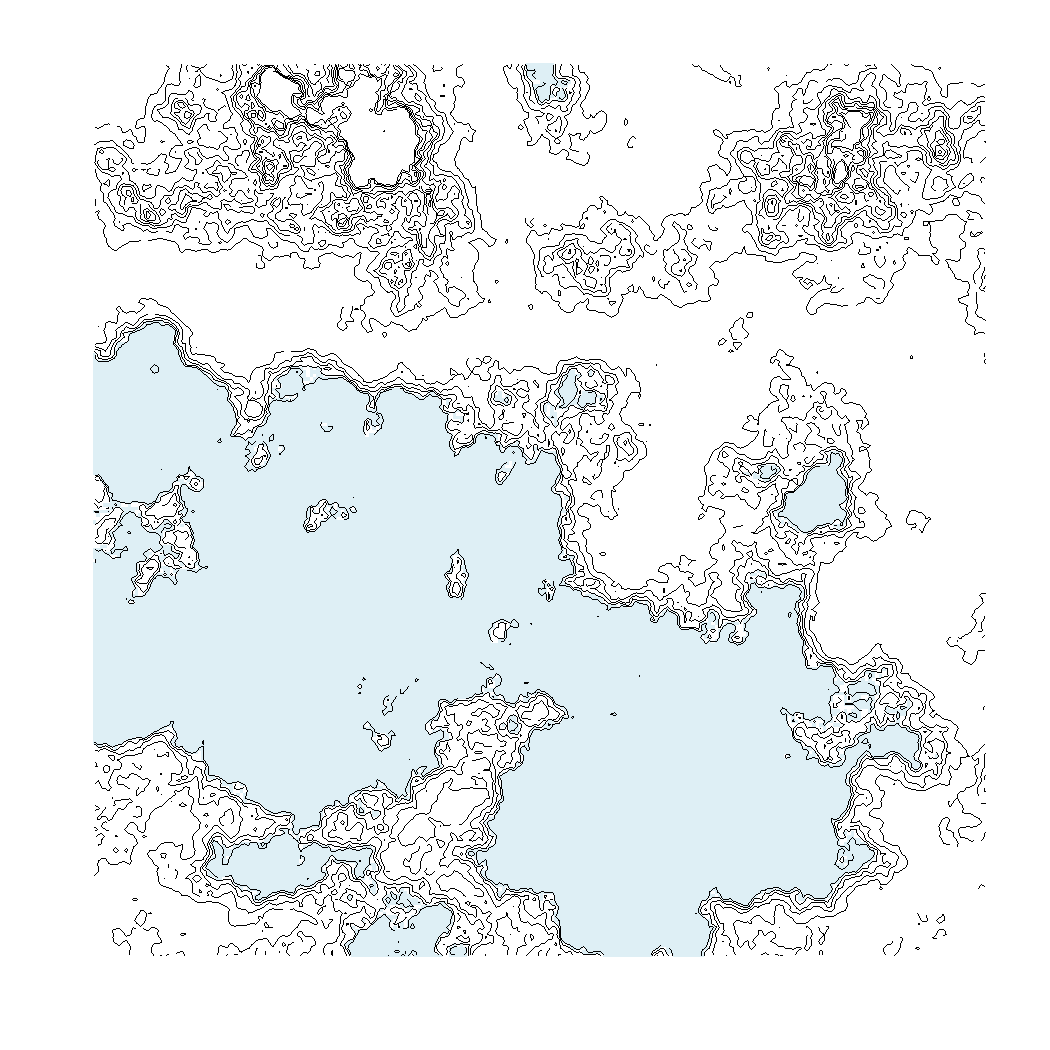
\includegraphics[width=.65\textwidth]{all}
    \caption{Map of rabbit with all published settlement}
    \label{fig:newage}
\end{figure}

\section{Method}
To show that we are right, we designed a powerfiulll mathematical tools, that we call: ``Test for Balanced Equilibrium``. This very clever use of mathematic, has never been used at our knowledge. Its power resides on the fact that it allows to show that are geographical areas  are basically in a peacufl equilibrium.

To do that we group the settlement in 4 groups: the two firs being the group from the old ages, the second the groups from the new ages 


\pagebreak

\section{Results}

\begin{figure}
    \centering
    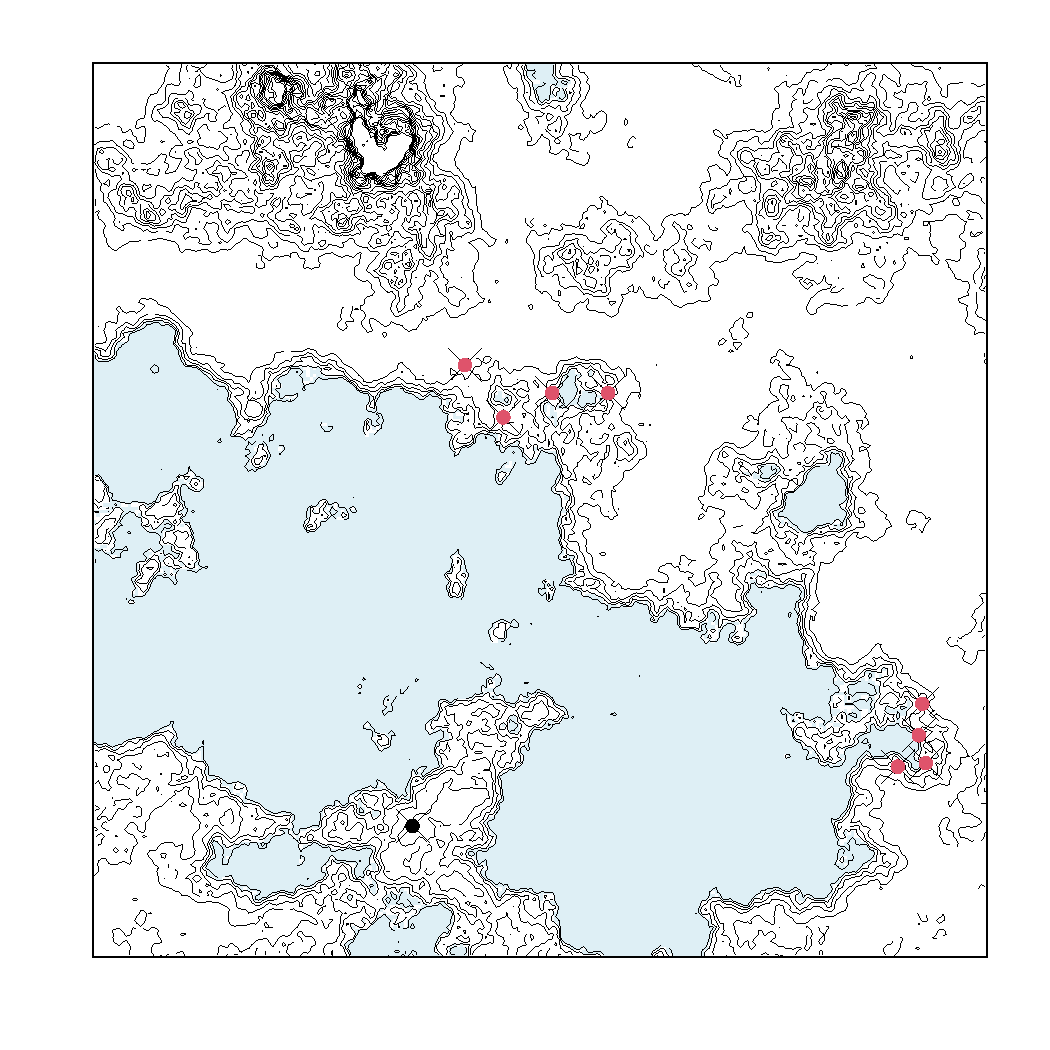
\includegraphics[width=.65\textwidth]{oldages}
    \caption{Map of rabbit hole during the Old age (~7200 - 7000 BP)  }
    \label{fig:newage}
\end{figure}

\begin{figure}
    \centering
    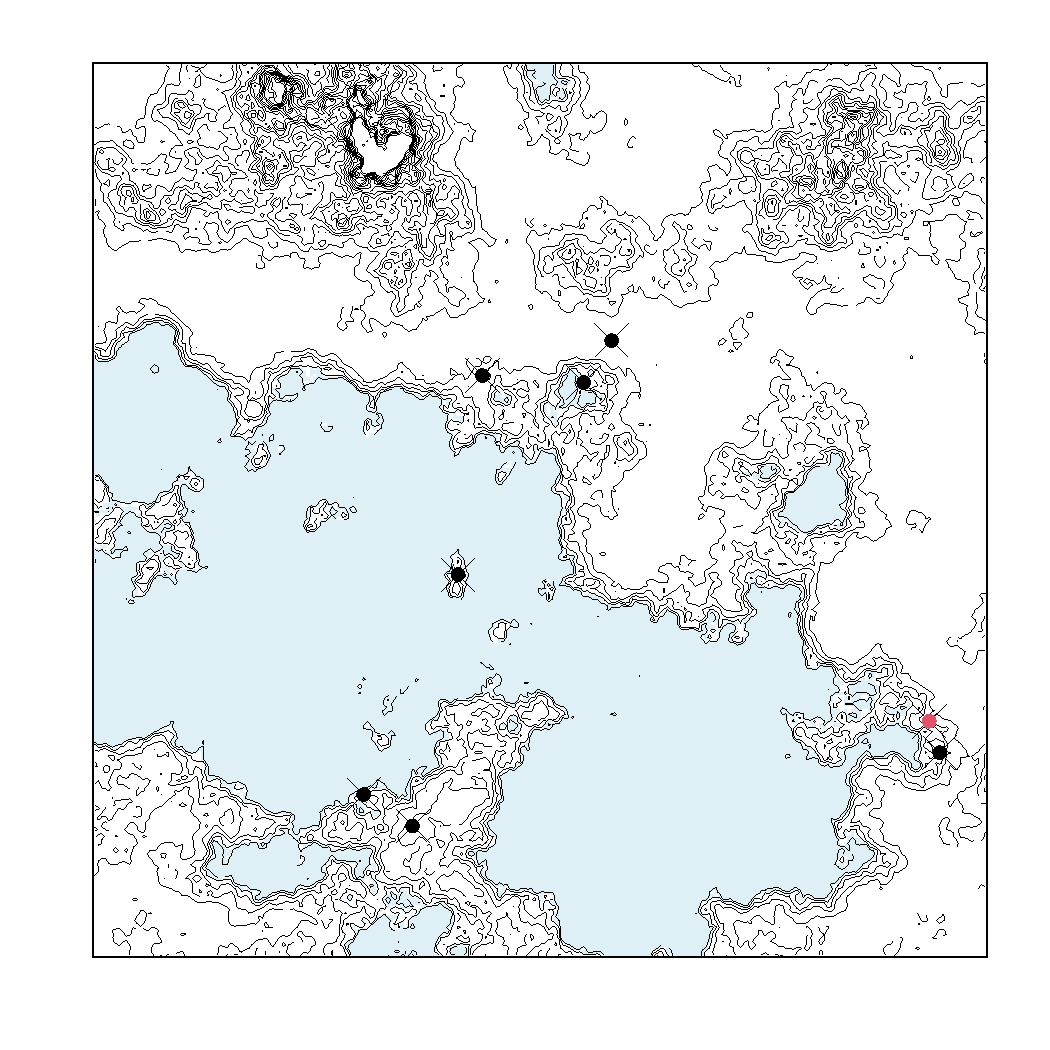
\includegraphics[width=.65\textwidth]{newages}
    \caption{Map of Rabbit hole after Farmer extension  (~7000 - 6800 BP)  }
    \label{fig:oldage}
\end{figure}
\begin{figure}
    \centering
    \makebox[\textwidth][c]{
    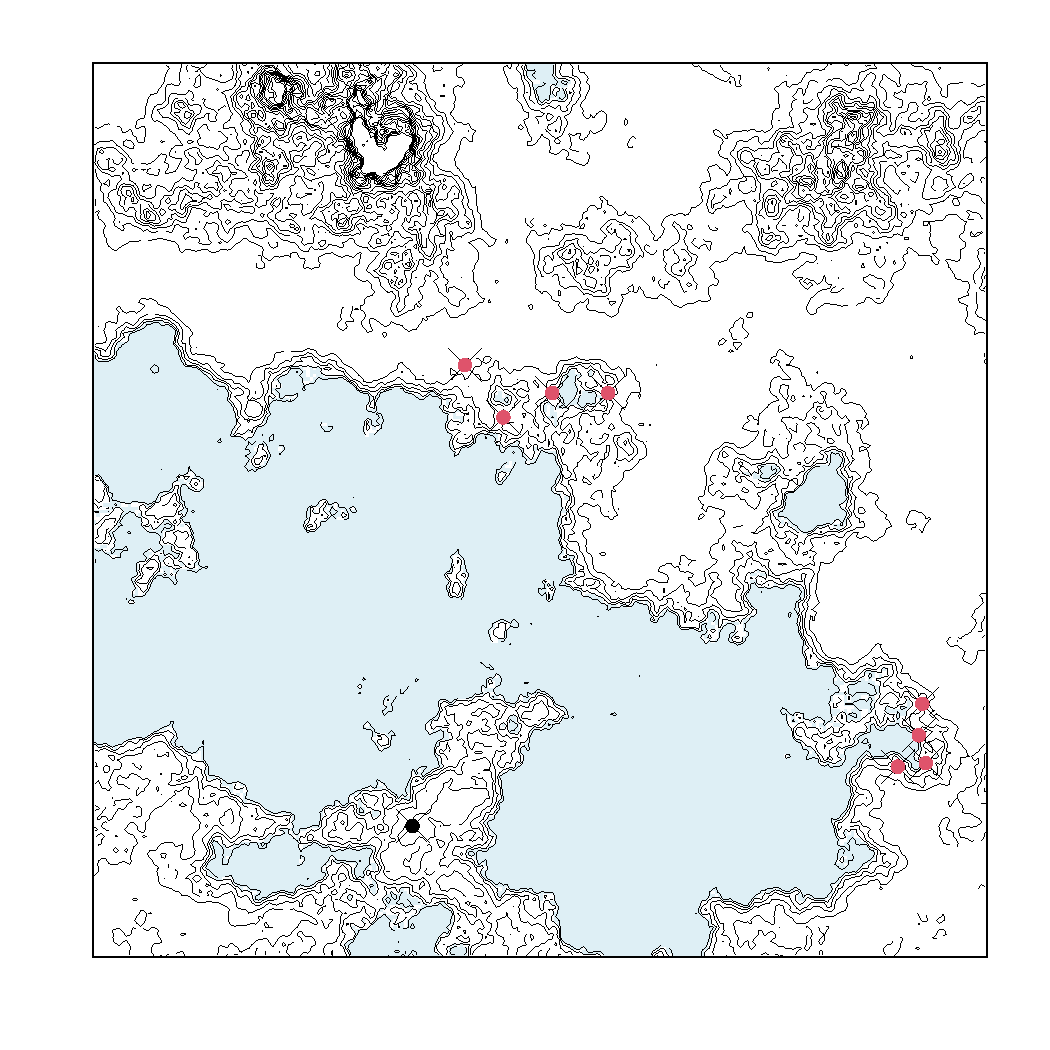
\includegraphics[width=.75\textwidth]{oldages}
    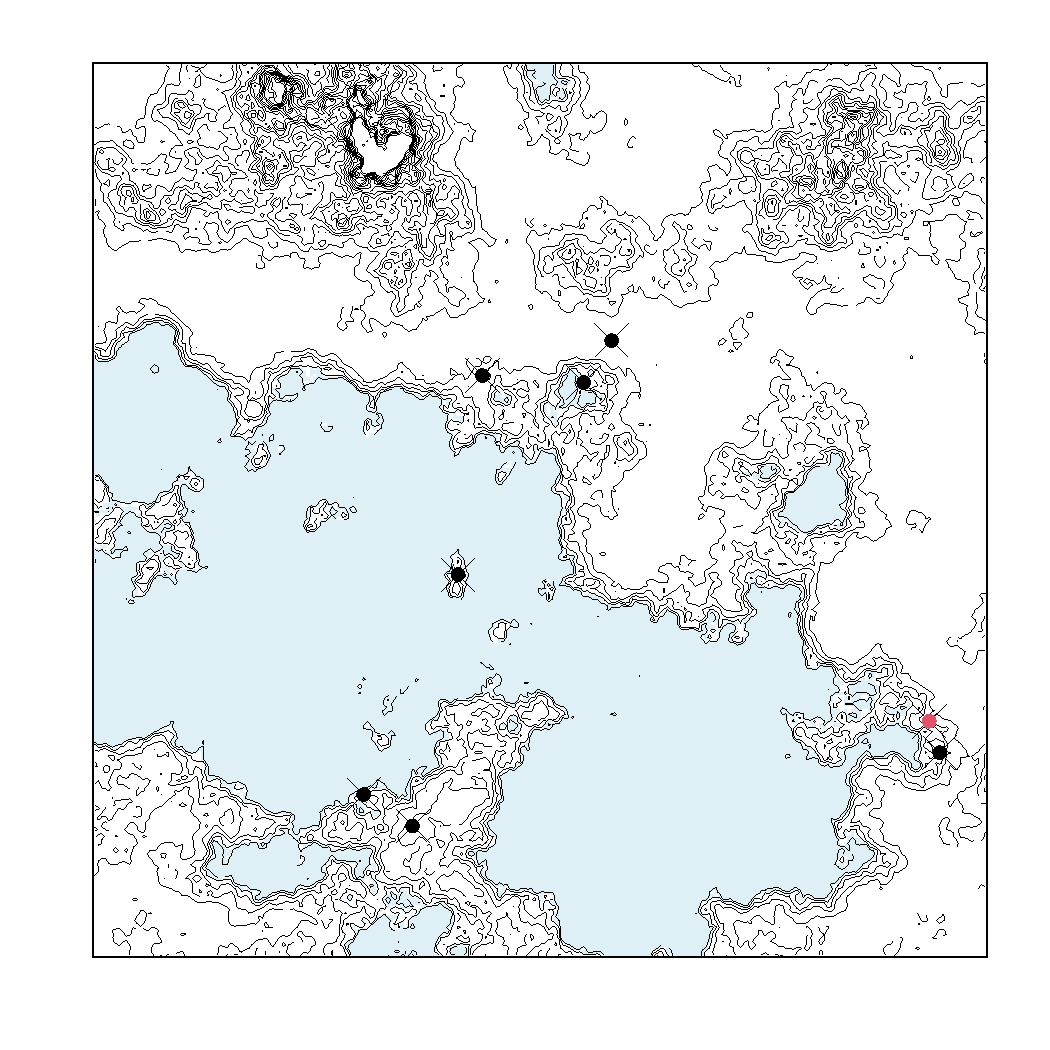
\includegraphics[width=.75\textwidth]{newages}
}
    \caption{Map of rabbit hole during the Old age (~7200 - 7000 BP) on the left, after Farmer extension  (~7000 - 6800 BP) on the right }
    \label{fig:twomaps}
\end{figure}
\end{document}

